\chapter{Аналитический раздел}

\section{Алгоритм шифрования <<RSA>>}

RSA --- криптографический алгоритм с открытым ключом, основывающийся на вычислительной сложности задачи факторизации.

Алгоритм:

\begin{enumerate}
	\item Выбираем два случайных простых числа $p$ и $q$.
	\item Вычисляем их произведение: $N = p \times q$.
	\item Вычисляем функцию Эйлера: $\phi(N) = (p - 1) \times (q - 1)$.
	\item Выбираем число $e$ (обычно простое, но необязательно), которое меньше $\phi(N)$ и является взаимно простым с $\phi(N)$.
	\item Ищем число $d$, обратное числу $e$ по модулю $\phi(N)$:
	\begin{equation*}
		d \times e \equiv 1 ~~ (\textrm{mod} ~~ \phi(N)).
	\end{equation*}

	Найти его можно через расширенный алгоритм Евклида.
\end{enumerate}

\section{Алгоритм хеширования <<MD5>>}

MD5 --- 128-битный алгоритм хеширования, разработанный профессором Рональдом Л. Ривестом из Массачусетского технологического института (Massachusetts Institute of Technology, MIT) в 1991 году.
Предназначен для создания «отпечатков» или дайджестов сообщения произвольной длины и последующей проверки их подлинности.
Широко применялся для проверки целостности информации и хранения хешей паролей, однако признан небезопасным из-за малой длины получаемого хэша и простотой самого алгоритма.

\chapter{Конструкторская часть}

\section{Разработка алгоритма}

На рисунке \ref{fig:algo} представлена схема создания и проверки цифровой подписи.

\begin{figure}[h!]
	\centering
	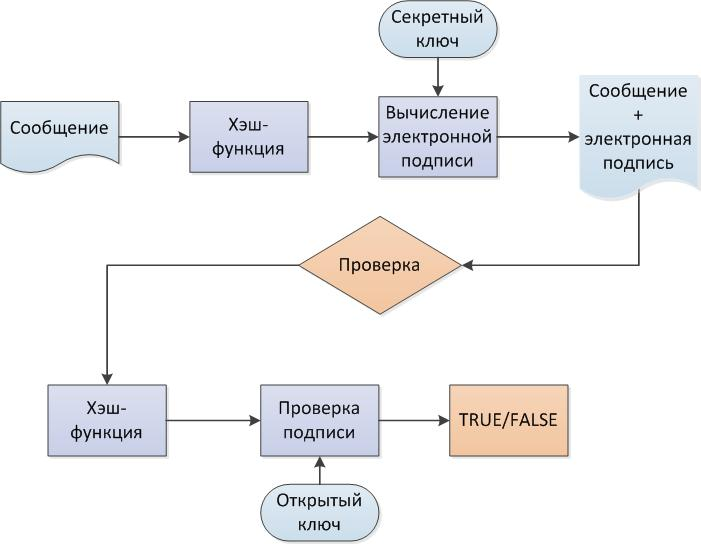
\includegraphics[width=0.85\textwidth]{img/RSA.jpeg}
	\caption{Схема создания и проверки цифровой подписи}
	\label{fig:algo}
\end{figure}
\clearpage
